

\chapter{Evaluation} \label{sect-evaluation}
In this chapter we use LIME, SHAP and Lucid (for image-based models) on various types of models to gain an understanding on how predictions on different model architectures are explained.

\section{House Prices}
We start off by training a \emph{Random Forest Regressor} for predicting house prices as introduced in section \ref{sect-intro-problem}. We make use of the  Boston Housing Dataset which contains US census data concerning houses in various areas around the city of Boston. Each sample corresponds to a unique area and has about a dozen measures. Alongside with price, the dataset also provides information such as Crime (CRIM), areas of non-retail business in the town (INDUS), the age of people who own the house (AGE), alongside many other attributes.  The dataset contains 506 samples where the target variable is the median value of owner-occupied homes in \$1000's (MEDV).

\subsection{LIME}
Figure \ref{fig:lime-house} is the explanation LIME provides for an area in Boston where the median price of housing was predicted to be 19870\$. From this Figure we are able to deduce that the feature that had the largest negative impact on the median price of this area is the \% lower status of the population (LSTAT) and the feature which had the largest positive impact is the average number of rooms per dwelling (RM).
\begin  {figure}[!htpb]
  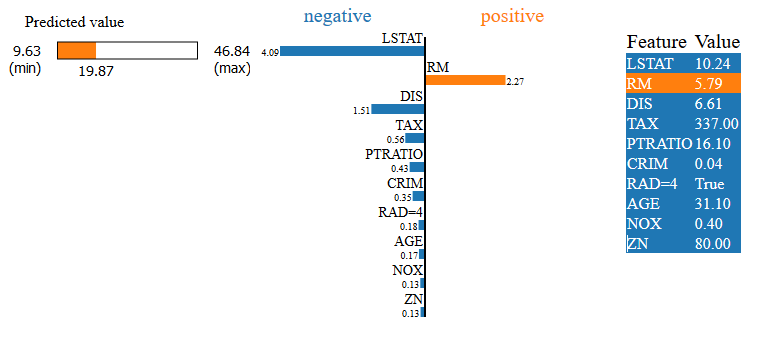
\includegraphics[width=\linewidth]{Evaluation_Images/House_LIME.png}
  \caption{LIME explanation for for a single area in Bostons median price.}
  \label{fig:lime-house}
\end{figure}
\subsection{SHAP}
Figure \ref{fig:shap-house-single} is the explanation SHAP provides for the same Boston area used in LIME. The base value is the average model output over the training dataset. The figure highlights how each feature contributes to pushing the prediction from the base value. The red values have a positive impact on the prediction and the blue values a negative impact. The explanation provided is a lot different to that of LIME's, because the SHAP values represent how each feature affects the base value.
\begin  {figure}[!htpb]
  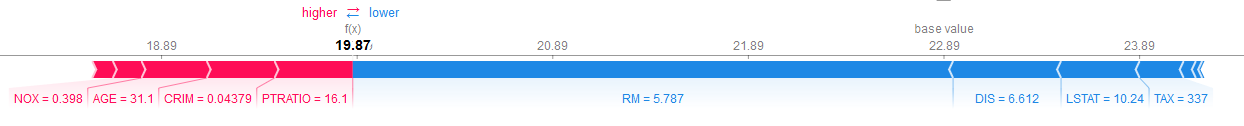
\includegraphics[width=\linewidth]{Evaluation_Images/house_indv_shap.png}
  \caption{SHAP explanation for a single area in Bostons median price.}
  \label{fig:shap-house-single}
\end{figure}
Figure \ref{fig:shap-house-entire} is the explanation that SHAP provides over multiple different areas . This is known as a summary plot and it compares SHAP values of multiple instances and how their impact on the model prediction is related to the magnitude of that feature. Features which have larger SHAP values increased the median price where as those with smaller SHAP values decreased the median price.
\begin  {figure}[!htpb]
  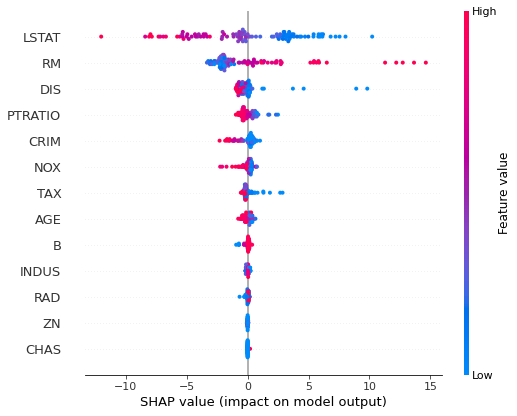
\includegraphics[width=\linewidth]{Evaluation_Images/house_shap.png}
  \caption{SHAP explanation over all the areas in Boston.}
  \label{fig:shap-house-entire}
\end{figure}
\section{MNIST}

The MNIST digit classification problem is one of the most popular machine learning problems in image processing. The dataset consists of \emph{60000} training images and \emph{10000} test images of handwritten digits with a size of $28\times28$. The goal is to determine what digit class \emph{0-9} the specific image belongs to.

\subsection{LIME}
Since there are $28 \times 28 = 784$ potential features, LIME creates a perturbed input $z^{'}$ by randomly choosing subsets of the non-zero features.  We limited the amount of samples created to 1000 for this problem. In Figure \ref{fig:lime-mnist} we can see for the specific handwritten digit \emph{5}, the green pixels represents pixels which attributed towards predicting the that the digit is 5 and red pixels which attributed towards the digit being 3.
\begin  {figure}[!htpb]
  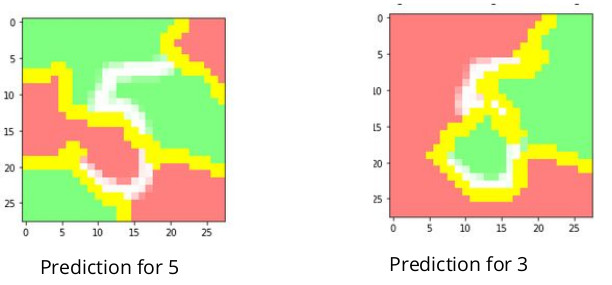
\includegraphics[width=\linewidth]{Evaluation_Images/Lime_mnist.jpg}
  \caption{Example of LIME visual feedback for the digit 5.}
  \label{fig:lime-mnist}
\end{figure}

\subsection{SHAP}
When making use of SHAP we are able to take an expectation of multiple samples in order to gain a more accurate representation of the attributed SHAP values, for this problem we took a set of 100 samples. In Figure \ref{fig:shap-mnist} we visualize the SHAP values over 4 different samples, for the 4 input images SHAP displays the SHAP values for the prediction to each class. The red masks are the pixels which attributed towards that class while the blue pixels attributed against that class.
\begin  {figure}[!htpb]
  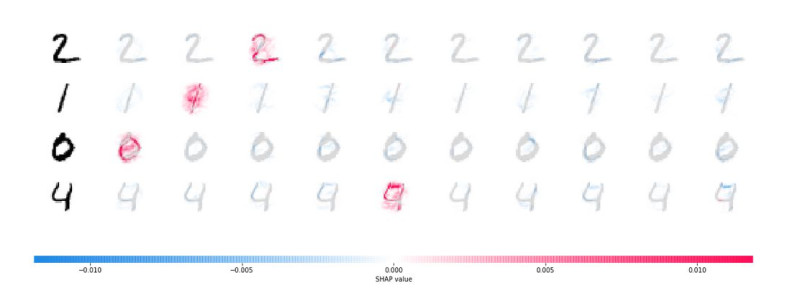
\includegraphics[width=\linewidth]{Evaluation_Images/Shap_mnist.jpg}
  \caption{SHAP values for 4 digits.}
  \label{fig:shap-mnist}
\end{figure}

\subsection{Lucid}
For Lucid we look at the spatial activations into two of the hidden convolutional layers labeled \emph{Conv2} and \emph{Conv3} respectively. Lucid provides a user interactive interface for viewing the activations, however in this example we will showcase static visual feedback. In Figure \ref{fig:lucid-mnist} for the two hidden layers \emph{Conv1} and \emph{Conv2} we are able to use spatial activations to see where and how much a specific set of pixels in the Conv1 Layer attributed in the target layer Conv2. The orange square is the set of pixels we are looking at in the starting layer and the whitened pixels in the target layer is where the activations happen

\begin  {figure}[!htpb]
  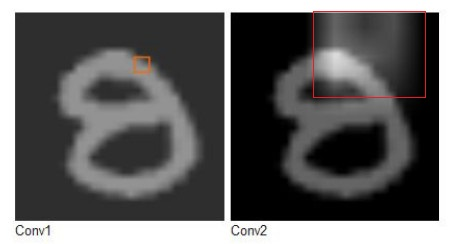
\includegraphics[width=\linewidth]{Evaluation_Images/Lucid_mnist.jpg}
  \caption{Lucid spatial activation for the digit 8.}
  \label{fig:lucid-mnist}
\end{figure} 

\section{Cats vs Dogs}

The Cats vs. Dogs is an image classification problem of finding suitable detectors for differentiating whether an image is of a cat or a dog. The dataset consists of 1000 \emph{training images} and  500 \emph{test images} with a size of $150\times150\times3$. 


\subsection{LIME}
 In Figure \ref{fig:lime-cat} we have an image of a cat and we visualize which super pixels attributed towards the \textbf{prediction of the image being a dog}, the green sections represent pixels that attributed towards being a dog where as the red sections represent pixels which attributed towards it being a cat. As a human this seems to make some intuitive sense, the ears of the cat are marked as negative attributions due to the fact that we associate dogs with ``droopy ears'', where as the cat has ``fluffy ears''.
\begin  {figure}[!htpb]
\centering
  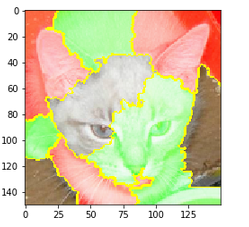
\includegraphics[width=0.8\linewidth]{Evaluation_Images/cats_explain.png}
  \caption{LIME on an image of a cat explaining which pixels attributed to it being a dog.}
  \label{fig:lime-cat}
\end{figure}

\subsection{SHAP}
In Figure \ref{fig:shap-cat} we show the SHAP values of 5 input samples and how they attributed towards whether the image is that of a cat or dog. SHAP provides much more detailed descriptions as each individual pixel is marked but LIME seems to be easier to understand as super-pixels are marked rather than individual ones. In figrue \ref{fig:shap-cat} we can see the SHAP values for 5 samples. The middle column is the attribution values for prediction towards being a cat, where as the right column is the attribution for being a dog. Red indicates a positive attribution, where as blue indicates a negative prediction.
\begin  {figure}[!htpb]
  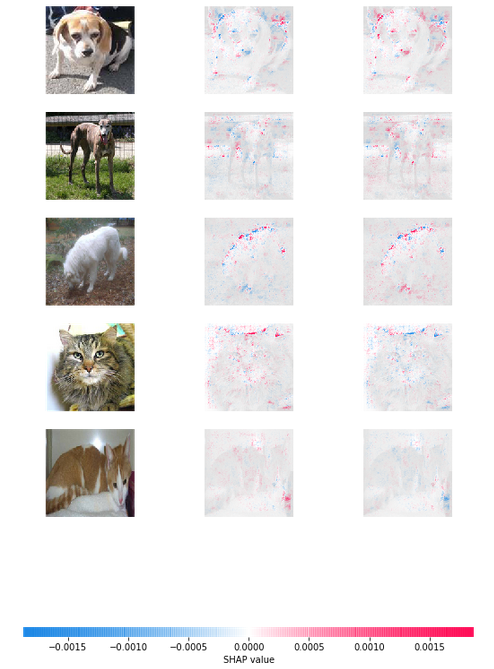
\includegraphics[width=\linewidth]{Evaluation_Images/CATS_DOGS_SHAP.png}
  \caption{Shap values for 5 different pictures of cats and dogs.}
  \label{fig:shap-cat}
\end{figure}

\subsection{Lucid}
In Figure \ref{fig:lucid-cat} we once again look at spatial activations between two hidden convolutional layers. However, in this case we included the gradient in the starting layer which shows the magnitude of the activations from the previous layers. In Figure \ref{fig:lucid-cat} for the two hidden layers \emph{Conv2} and \emph{Conv3} we are able to use spatial activations to see where how much a specific set of pixels in the Conv2 Layer attributed in the target layer Conv3. The orange square is the set of pixels we are looking at in the starting layer and the whitened pixels in the target layer is where the activations happen.
\begin  {figure}[!htpb]
  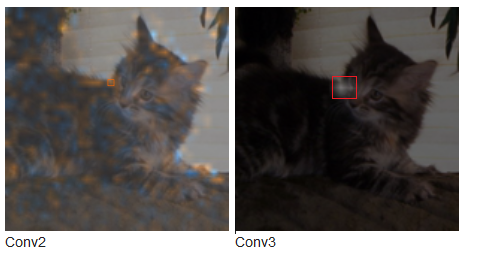
\includegraphics[width=\linewidth]{Evaluation_Images/LUCID_CATS_DOGS_2_v2.png}
  \caption{Lucid spatial activations between two layers in an image of a cat.}
  \label{fig:lucid-cat}
\end{figure}

\section{IMDB Sentiment analysis}
The goal of the \emph{IMDB sentiment analysis} problem is to classify whether a movie review is positive or negative. The dataset consists 25000 \emph{training} samples and 25000 \emph{tests sample} where is sample is a vector of size $80\times1$. Each sample is a word embedding representing which words are present and in what order.

\subsection{LIME}
In Figure \ref{fig:lime-imdb} an attribution value is given to each individual word in the review, in this example we only show 10 words which had the largest impact. The model predicted that the review was negative, some words such as ``of'' and ``with'' by human understanding does not inherently have negative connotations, however in the context of this review it was shown that it was likely paired with negative words such as ``lies''. Due to domain knowledge being needed, there is always some human interaction and if we have thousands of words that we are attributing on, it may become difficult to understand.
\begin  {figure}[!htpb]
  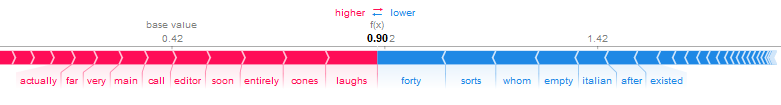
\includegraphics[width=\linewidth]{Evaluation_Images/IMDB_explanation_1.png}
  \caption{The results of the attribution where the words which had the most impact towards the prediction are sorted by magnitude. Blue represents it being a negative review and orange represents positive.}
  \label{fig:lime-imdb}
\end{figure}


\subsection{SHAP}
In Figure \ref{fig:shap-imdb} we have chosen \emph{positive} to be the primary class of prediction. In this case SHAP orders the words by magnitude of attribution and the left side indicated words that attributed towards (increased the probability) of the primary class and the right side indicates words which attributed against (decreased the probability) the primary class. Since the predicted class was \emph{negative} we can see how the negative attributions outweighed the positive attributions resulting in an output class of negative.

\begin  {figure}[!htpb]
  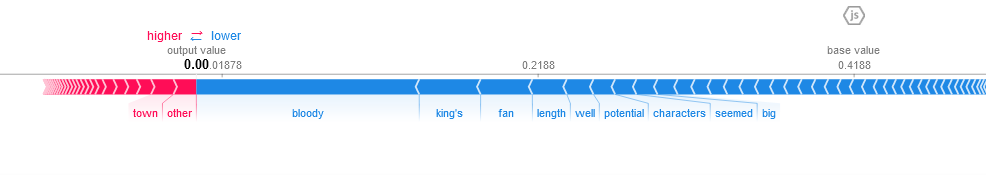
\includegraphics[width=\linewidth]{Evaluation_Images/SHAP_IMDB.png}
  \caption{The output value for this particular case was 0.00 which means we have predicted that the review is negative. The red words and words which attributed towards the review being positive, where as the blue words attributed towards the review being negative sorted by magnitude.}
  \label{fig:shap-imdb}
\end{figure}

\section{Provide intuition into LIME and SHAP}

In this section we attempt to gain intuition into LIME and SHAP by showing the relationship between a model with predefined weights and the produced feature attributions. 
\subsection{Setup}
 We start by creating a model with 5 weights which  are explicitly defined as,
\begin{align*}
w_1 = 5,\ w_2 = 3,\ w_3 = 4,\ w_4 = 9,\ w_5 = 1,
\end{align*}
in order to see the importance ratios between the weights we normalize them to unity,
\begin{align*}
    w_1 = 0.227, \ w_2 = 0.136, \ w_3 =  0.18 ,\ w_4 = 0.409, \ w_5 = 0.045.
\end{align*}
The next step is generating 500 synthetic data samples where each sample is an integer vector with 5 values between 1 and 100. We then assign each sample a probability of belonging to one of two respective classes \emph{Positive} and \emph{Negative} which are calculated as follows,
\begin{flalign*}
\begin{split}
\mbox{Sum(Positive)} &= X[0] \times w_1 + X[1] \times  w_2 + X[2] \times  w_3,
\\
\mbox{Sum(Negative)} &= X[3] \times  w_4 + X[4] \times  w_5 ,
\end{split}
\end{flalign*}
\begin{flalign*}
\begin{split}
\mbox{Prob(Positive)} &= \frac{Sum(Positive)}{Sum(Positive) + Sum(Negative)},
\\
\mbox{Prob(Negative)} &= \frac{Sum(Negative)}{Sum(Positive) + Sum(Negative)},
\end{split}
\end{flalign*}
where $X$ is the feature vector and $X[i]$ represents the feature at index $i$.
We pass this synthetic data to LIME and SHAP and observe how faithfully their produced feature attributions are to the actual weights.
\subsection{LIME}
Let $X_{1}$ and $X_{2}$ be 2 inputs with the following feature values,
\begin{flalign*}
\begin{split}
    X_1 &= [8,\ 24,\ 67,\ 87,\ 79],
    \\
    X_2 &= [48,\ 10,\ 94,\ 52,\ 98],
    \end{split}
\end{flalign*}
calculating the class probabilities for $X_1$,
\begin{flalign*}
\begin{split}
   \mbox{Prob(Positive)} &= 0.30595813,
    \\
    \mbox{Prob(Negative)} &= 0.6940418,
    \end{split}
\end{flalign*}
and for $X_2$,
\begin{flalign*}
\begin{split}
    \mbox{Prob(Positive)} &=  0.5330033 ,
    \\
    \mbox{Prob(Negative)} &= 0.4669967,
    \end{split}
\end{flalign*}
therefore $X_1$ belongs to the \emph{Negative} class and $X_2$ to the \emph{Positive} class.
We pass these two inputs to the Tabular Explainer of LIME in order to extract the feature attributions from the explanations. The visualization produced by LIME shows the feature attributions rounded to 2 significant digits, however for better accuracy the comparisons will use 3 significant digits. In Figure \ref{fig:lime-ground} we can see the attribution values which LIME assigns to each class for instance $X_1$,
\begin{align*}
    \phi_1 = 0.069, \ \phi_2 = 0.042, \ \phi_3 = 0.056 ,\ \phi_4 = 0.11, \ \phi_5 = 0.013,
\end{align*}
normalizing to unity,
\begin{align*}
    \phi_1 = 0.238, \ \phi_2 = 0.145, \ \phi_3 = 0.192 ,\ \phi_4 = 0.379, \ \phi_5 = 0.046.
\end{align*}
The explanation for $X_2$ can be seen in Figure \ref{fig:lime-ground2} and the attribution values are,
\begin{align*}
    \phi_1 = 0.061, \ \phi_2 = 0.036, \ \phi_3 = 0.048 ,\ \phi_4 = 0.126, \ \phi_5 = 0.014,
\end{align*}
normalizing to unity,
\begin{align*}
    \phi_1 = 0.215, \ \phi_2 = 0.127, \ \phi_3 = 0.167 ,\ \phi_4 = 0.441, \ \phi_5 = 0.05.
\end{align*}
\begin  {figure}[!htpb]
  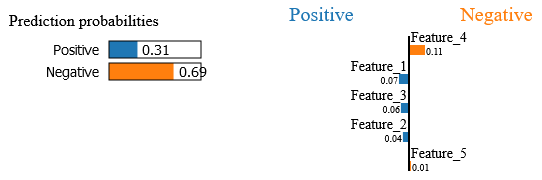
\includegraphics[width=\linewidth]{Evaluation_Images/lime-ground.png}
   \caption{LIME explanation for input $X_1$}
    \label{fig:lime-ground}
\end{figure}
\begin  {figure}[!htpb]
  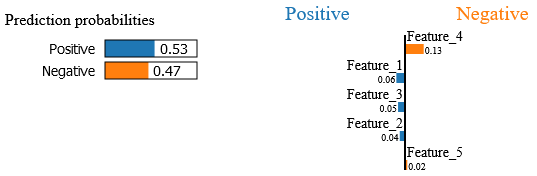
\includegraphics[width=\linewidth]{Evaluation_Images/lime-ground2.png}
   \caption{LIME explanation for input $X_2$}
    \label{fig:lime-ground2}
\end{figure}
A limitation of LIME that we have discussed before is that it only explains a single prediction at a time and we can see from the differences between the attributions values of $X_1$ and $X_2$  that there is variance between instances. This issue could be circumvented by  explaining multiple instances and averaging over the results.


\subsection{SHAP}
SHAP allows us to use the entire training set of 500 samples as background samples and gain attribution values which are averaged over the entire data set. We use \emph{Kernel SHAP} for this experiment since our model is not a Neural Network. The feature attribution values that we have derived from SHAP and normalized to unity are,
 \begin{align*}
    \phi_1 = 0.211, \ \phi_2 = 0.126, \ \phi_3 = 0.167 ,\ \phi_4 = 0.44, \ \phi_5 = 0.057.
\end{align*}
Figure \ref{fig:shap-ground} shows how each feature contributed towards the models prediction over the entire dataset for the \emph{Positive} class. The more red a point is the higher that particular feature value was, where as more blue indicates a lower value. The x-axis indicates the SHAP value, where the higher the value is the more that particular feature attributed towards the probability of the \emph{Positive} class and the lower it is the more it attributed against it. From this Figure we can see that Feature 1 to 3 attributed towards the \emph{Positive} class with Feature 1 attributing the most and Feature 2 the least. We can also see that Feature 4 attributed the most against it and Feature 5 the least. These results are inline with how we have defined the weights and from this graph we are able to visualize the different attributions between samples and their variances.
\begin  {figure}[!htpb]
  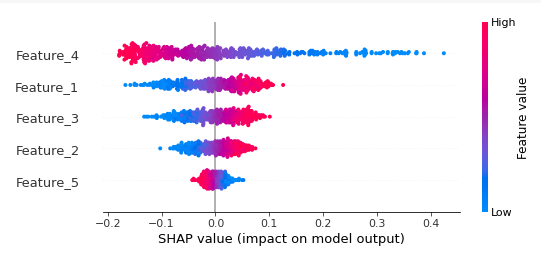
\includegraphics[width=\linewidth]{Evaluation_Images/shap_ground.png}
\caption{SHAP explanation for our chosen input $X_1$}
 \label{fig:shap-ground}
\end{figure}

\subsection{Comparison}
We have tabulated the results for comparison purposes in Figure \ref{fig:weight-tab}. We have also graphed the weights and attributions in Figure \ref{fig:weight-graph} for better visualization.We can see that the attribution values are fairly accurate in describing the defined weights and the ratios of feature importance are comparable to those of our model. From the results we have gathered, we can conclude that LIME and SHAP are able to generate fairly accurate linear estimations of a linear model by only using it's prediction results. These results allow us to gain some trust in LIME and SHAP, however further experimentation is needed to see if complex neural networks can also be approximated well.
\begin  {figure}[!htpb]
  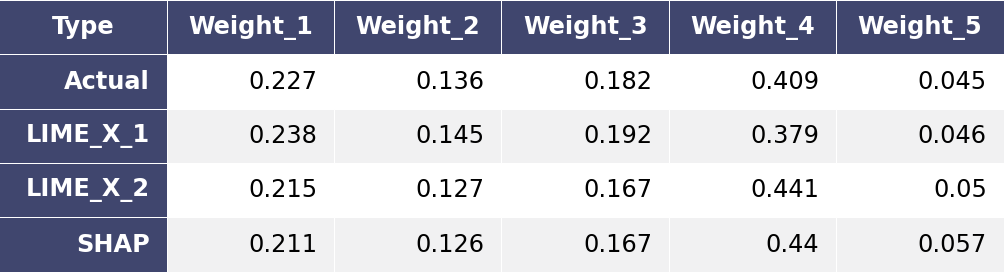
\includegraphics[width=\linewidth]{Evaluation_Images/weight_table.png}
   \caption{Comparison of weights.}
    \label{fig:weight-tab}
\end{figure}

\begin  {figure}[!htpb]
  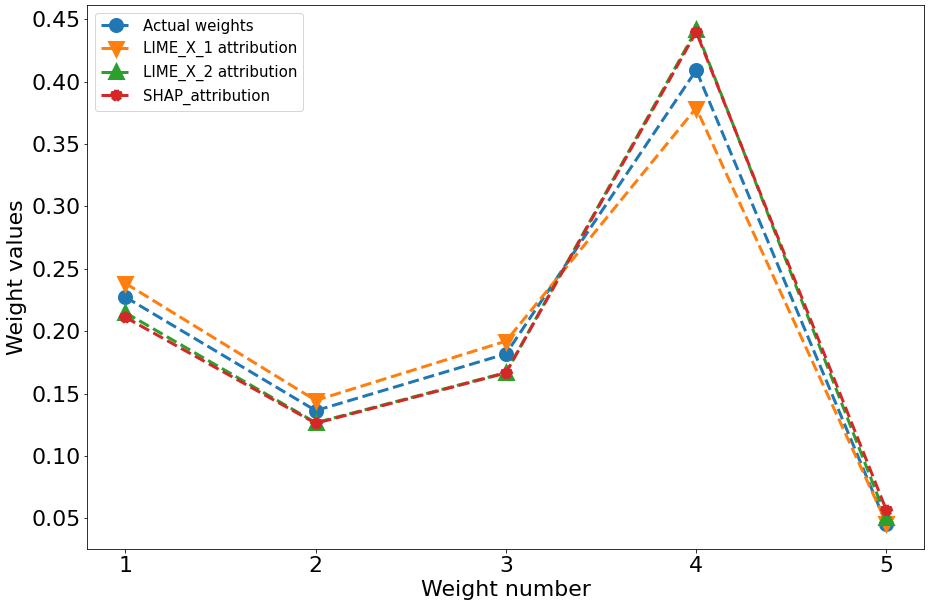
\includegraphics[width=\linewidth]{Evaluation_Images/weight_comp.png}
   \caption{Graph of weights.}
    \label{fig:weight-graph}
\end{figure}



